\section {Nível de Portfólio}

A divisão em camadas do SAFe proporciona uma visão ampla de todos os níveis de requisitos que devem ser tratados. A camada Portifólio abrange os requisitos a nível de negócio, ou seja, uma visão com alto nível de abstração. De acordo com o nosso processo, o nível de portifólio visto na (Figura \ref{img:portfolio}) possui as seguintes tarefas:

\begin{itemize}
\item Analisar a empresa Eletrojun.
\item Compreender as necessidades da empresa.
\item Identificar conjunto de épicos.
\item Priorizar épico.
\item Gerenciar épicos.
\end{itemize}

\FloatBarrier
\begin{figure}[!htpd]
		\centering
		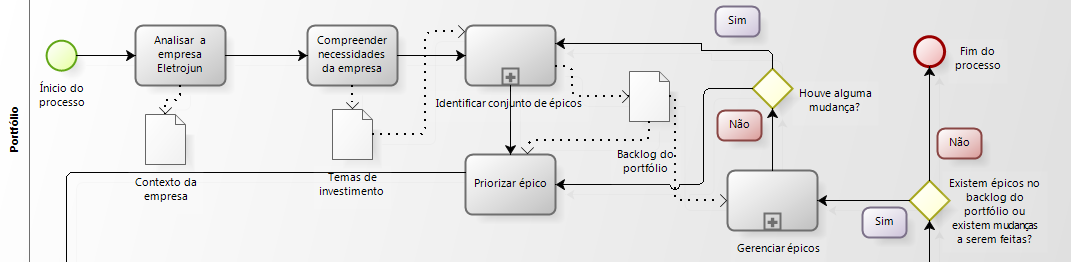
\includegraphics[scale=0.4]{figuras/portfolio}
		\label{img:portfolio}
		\caption{Processo à nível de Portfólio}
\end{figure}
\FloatBarrier

As tarefas listadas foram cumpridas com o auxílio das técnicas de elicitação, Brainstorm e Entrevista. As atas de reunião, juntamente com as entrevistas, podem ser encontradas no apêndice XX.

\subsection {Backlog Portfólio}

\textbf{Tema de Investimento:} Gestão e desenvolvimento de projetos.

 A partir das prioridades da organização, identificou-se que a empresa desejava investir na Gerência e Desenvolvimento de novos projetos. Este tema de investimento tem a função de fomentar o desenvolvimento de novos projetos por parte dos alunos da FGA, tendo como principal característica a necessidade de um meio que una os estudantes e crie um ambiente favorável para o desenvolvimento de ideias e projetos.

Para a especificação dos épicos utilizou-se o padrão recomendado pelo SAFe [SAFe 2015], que é o template  \textit{lightweight business case}.

\textbf{Épico 01 - EP-01:} Gerenciamento de Usuários: Abrange todas as ações de administração dos usuários do sistema, desde o cadastro de um usuário até a sua exclusão do sistema.

\textbf{Épico 02 - EP-02:} Gerenciamento de Projetos: Abrange todas as ações de administração de projetos no sistema, desde a sua publicação até o seu cumprimento total.

\textbf{Épico 03 - EP-03:} Gerenciamento de Atividades: Abrange todas as ações de administração e gerenciamento de atividades pontuais, dentro e fora dos projetos.

\textbf{Épico 04 - EP-04:} Gerenciamento de Premiações: Abrange todas as ações manutenção de premiações aos usuários do sistema.

\FloatBarrier
\begin{table}[!htpd]
\centering
\caption{Épico  1}
\label{my-label}
\begin{tabular}{|l|l|l|}
\hline
\multicolumn{3}{|l|}{\textbf{Caso de Negócio}}                                                                                                                                                                                                                                                                                                   \\ \hline
\textbf{Para}                     & \multicolumn{2}{l|}{Os alunos e profissionais do Campus Gama}                                                                                                                                                                                                                                                \\ \hline
\textbf{Que}                      & \multicolumn{2}{l|}{Possuem projetos e desejam compartilhar as suas ideias}                                                                                                                                                                                                                                  \\ \hline
\textbf{O}                        & \multicolumn{2}{l|}{Gerenciamento de usuários}                                                                                                                                                                                                                                                               \\ \hline
\textbf{É uma}                    & \multicolumn{2}{l|}{\begin{tabular}[c]{@{}l@{}}Ferramenta que permite a realização de,procedimentos de administração \\ e manutenção de usuários\end{tabular}}                                                                                                                                               \\ \hline
\textbf{Que}                      & \multicolumn{2}{l|}{\begin{tabular}[c]{@{}l@{}}Possibilita o gerenciamento e pleno controle da conta de usuário, bem \\ como a interação direta (adicionar/seguir) outro usuário\end{tabular}}                                                                                                               \\ \hline
\textbf{Diferente}                & \multicolumn{2}{l|}{\begin{tabular}[c]{@{}l@{}}Da Situação atutal onde não há um controle de membros colaborativos \\ nos diversos projetos em execução do Campus Gama\end{tabular}}                                                                                                                         \\ \hline
\textbf{Nossa Solução}            & \multicolumn{2}{l|}{\begin{tabular}[c]{@{}l@{}}Possibilita o cadastro e consequentemente um controle e interação de \\ usuários na plataforma\end{tabular}}                                                                                                                                                  \\ \hline
\multicolumn{3}{|l|}{\textbf{Escopo}}                                                                                                                                                                                                                                                                                                            \\ \hline
\textbf{Critérios de Sucesso}     & \multicolumn{2}{l|}{\begin{tabular}[c]{@{}l@{}}Usuários conseguem se cadastrar e manter sua conta de forma a \\ possibilitar interação (adicionar/seguir) usuários e pleno acesso às \\ funcionalidades da  ferramenta. \\ O administrador da ferramenta consegue gerenciar os usuários \\ do sistema.\end{tabular}} \\ \hline
\textbf{No Escopo}                &
	\multicolumn{2}{l|}{\begin{tabular}[c]{@{}l@{}}Cadastro, manutenção, administração e interação de usuários \\ (adicionar/seguir). \end{tabular}}  \\ \hline
\textbf{Fora do Escopo}           & \multicolumn{2}{l|}{Controle das atividades dos usuários dentro de um projeto}                                                                                                                                                                                                                               \\ \hline
\end{tabular}
\end{table}
\FloatBarrier

\FloatBarrier
\begin{table}[!htpd]
\centering
\caption{Épico 2}
\label{my-label}
\begin{tabular}{|l|l|l|}
\hline
\multicolumn{3}{|l|}{\textbf{Caso de Negócio}}                                                                                                                                                                                                                                                                                                                                                              \\ \hline
\textbf{Para}                     & \multicolumn{2}{l|}{\begin{tabular}[c]{@{}l@{}}Usuários administradores de projetos dentro da plataforma, \\ bem como seus  colaboradores\end{tabular}}                                                                                                                                                                                                                  \\ \hline
\textbf{Que}                      & \multicolumn{2}{l|}{Criam e administram a execução dos projetos}                                                                                                                                                                                                                                                                                                        \\ \hline
\textbf{O}                        & \multicolumn{2}{l|}{Gerencimento de Projetos}                                                                                                                                                                                                                                                                                                                           \\ \hline
\textbf{É uma}                    &
\multicolumn{2}{l|}{\begin{tabular}[c]{@{}l@{}}Ferramenta de automação de procedimentos de administração de \\ projetos\end{tabular}}                                                                                                                                                                                                                                                                              \\ \hline
\textbf{Que}                      & \multicolumn{2}{l|}{Facilita e agiliza o desenvolvimento colaborativo de projetos}                                                                                                                                                                                                                                                                                      \\ \hline
\textbf{Diferente}                & \multicolumn{2}{l|}{\begin{tabular}[c]{@{}l@{}}Da situação atual onde não há uma plataforma colaborativa de \\ desenvolvimento de projetos do Campus Gama\end{tabular}}                                                                                                                                                                                                 \\ \hline
\textbf{Nossa Solução}            & \multicolumn{2}{l|}{\begin{tabular}[c]{@{}l@{}}Automatizar os procedimentos de controle e administração dos\\ projetos em uma plataforma de integração\end{tabular}}                                                                                                                                                                                                    \\ \hline
\multicolumn{3}{|l|}{\textbf{Escopo}}                                                                                                                                                                                                                                                                                                                                                                       \\ \hline
\textbf{Critérios de Sucesso}     & \multicolumn{2}{l|}{\begin{tabular}[c]{@{}l@{}}Aumento da produtividade e integração dos alunos de forma \\ significativa, assim como a organização do projeto;\\ Usuários conseguem cadastrar projetos e executar todas as demais \\ tarefas referentes a ele; \\ Administrador da ferramenta consegue gerenciar os projetos  \\ cadastrados na ferramenta.\end{tabular}} \\ \hline
\textbf{No Escopo}                &
\multicolumn{2}{l|}{\begin{tabular}[c]{@{}l@{}}Criar, manter, administrar e acompanhar projetos em execução \\ na plataforma \end{tabular}}                                                                                                                                                                                                                                                                         \\ \hline
\textbf{Fora do Escopo}           & \multicolumn{2}{l|}{\begin{tabular}[c]{@{}l@{}}Interação entre usuários individuais, bem como bate-papo, sistema \\ de busca e manutenção de usuários.\end{tabular}}                                                                                                                                                                                                    \\ \hline
\end{tabular}
\end{table}
\FloatBarrier

\FloatBarrier
\begin{table}[!htpd]
\caption{Épico 3}
\label{my-label}
\begin{tabular}{|l|l|l|}
\hline
\multicolumn{3}{|l|}{\textbf{Caso de Negócio}}                                                                                                                                                                                                                 \\ \hline
Para                             & \multicolumn{2}{l|}{\begin{tabular}[c]{@{}l@{}}Todos os usuários da plataforma, tanto em perfil colaborador \\ como administrador de projeto\end{tabular}}                                                                                  \\ \hline
Que                              & \multicolumn{2}{l|}{Está em interação com projetos ou outros usuários}                                                                                                                                                                      \\ \hline
O                                & \multicolumn{2}{l|}{Gerenciamento de Atividades}                                                                                                                                                                                            \\ \hline
É uma                            & \multicolumn{2}{l|}{Conjunto de utilitários do sistema}                                                                                                                                                                                     \\ \hline
Que                              & \multicolumn{2}{l|}{\begin{tabular}[c]{@{}l@{}}Permite atividades de busca, venda, notificação e comunicação \\ dentro da ferramenta\end{tabular}}                                                                                          \\ \hline
Diferente                        & \multicolumn{2}{l|}{\begin{tabular}[c]{@{}l@{}}Da situação atual onde não há possibilidade de realizar todas \\ as atividades de um projeto em um sistema só\end{tabular}}                                                                  \\ \hline
Nossa Solução                    & \multicolumn{2}{l|}{\begin{tabular}[c]{@{}l@{}}Permite a realização de atividades que facilitam a dinamicidade \\ da plataforma colaborativa\end{tabular}}                                                                                  \\ \hline
\multicolumn{3}{|l|}{\textbf{Escopo}}                                                                                                                                                                                                                              \\ \hline
Critérios de Sucesso             & \multicolumn{2}{l|}{\begin{tabular}[c]{@{}l@{}}Aumentar consideravelmente a usabilidade do sistema, bem como \\ a navegabilidade e integração entre usuários;\\ Proporcionar ainda um sistema funcional de vendas de projetos\end{tabular}} \\ \hline
No Escopo                        & \multicolumn{2}{l|}{Bate-papo, venda, pesquisa, sistema de ajuda e notificação no sistema.}                                                                                                                                                 \\ \hline
Fora do Escopo                   & \multicolumn{2}{l|}{Gerenciamento de usuários e projetos dentro da plataforma.}                                                                                                                                                             \\ \hline
\end{tabular}
\end{table}
\FloatBarrier

\FloatBarrier
\begin{table}[!htpd]
\caption{Épico 4}
\label{my-label}
\begin{tabular}{|l|l|l|}
\hline
\multicolumn{3}{|l|}{\textbf{Caso de Negócio}}                                                                                                                                                                                                                                  \\ \hline
\textbf{Para}                     & \multicolumn{2}{l|}{\begin{tabular}[c]{@{}l@{}}Todos os usuários da plataforma, tanto em perfil colaborador como \\ administrador de projeto\end{tabular}}                                                                                  \\ \hline
\textbf{Que}                      & \multicolumn{2}{l|}{Está em interação com projetos ou outros usuários}                                                                                                                                                                      \\ \hline
\textbf{O}                        & \multicolumn{2}{l|}{Gerenciamento de Atividades}                                                                                                                                                                                            \\ \hline
\textbf{É uma}                    & \multicolumn{2}{l|}{Conjunto de utilitários do sistema}                                                                                                                                                                                     \\ \hline
\textbf{Que}                      & \multicolumn{2}{l|}{\begin{tabular}[c]{@{}l@{}}Permite atividades de busca, venda, notificação e comunicação dentro \\ da ferramenta\end{tabular}}                                                                                          \\ \hline
\textbf{Diferente}                & \multicolumn{2}{l|}{\begin{tabular}[c]{@{}l@{}}Da situação atual onde não há possibilidade de realizar todas as \\ atividades de um projeto em um sistema só\end{tabular}}                                                                  \\ \hline
\textbf{Nossa Solução}            & \multicolumn{2}{l|}{\begin{tabular}[c]{@{}l@{}}Permite a realização de atividades que facilitam a dinamicidade da \\ plataforma colaborativa\end{tabular}}                                                                                  \\ \hline
\multicolumn{3}{|l|}{\textbf{Escopo}}                                                                                                                                                                                                                                           \\ \hline
\textbf{Critérios de Sucesso}     & \multicolumn{2}{l|}{\begin{tabular}[c]{@{}l@{}}Aumentar consideravelmente a usabilidade do sistema, bem como a \\ navegabilidade e integração entre usuários.\\ Proporcionar ainda um sistema funcional de vendas de projetos\end{tabular}} \\ \hline
\textbf{No Escopo}                & \multicolumn{2}{l|}{Bate-papo, venda, pesquisa, sistema de ajuda e notificação no sistema}                                                                                                                                                 \\ \hline
\textbf{Fora do Escopo}           & \multicolumn{2}{l|}{Gerenciamento de usuários e projetos dentro da plataforma.}                                                                                                                                                             \\ \hline
\end{tabular}
\end{table}
\FloatBarrier

\section {Backlog Programa}

A camada de programa é a camada intermediária do processo. Este nível é responsável por identificar requisitos concretos e estabelecer estratégias para a implementação da solução. O nível de programa (Figura \ref{img:programa}) possui as seguintes atividades:

\begin{itemize}
\item Levantar Features
\item Identificar requisitos não-funcionais
\item Definir Roadmap
\item Priorizar Features
\item Planejamento da Release
\item Gerenciar Features
\item Planejamento da Release
\end{itemize}

\FloatBarrier
\begin{figure}[!htpd]
		\centering
		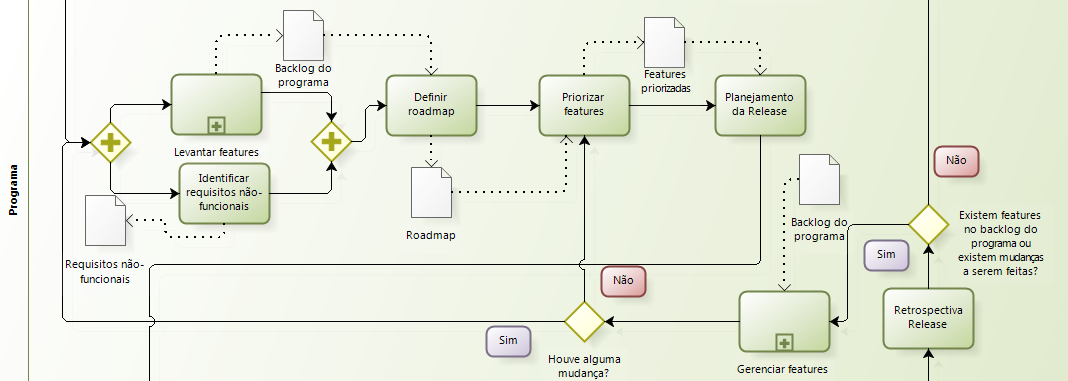
\includegraphics[scale=0.4]{figuras/programa}
		\label{img:programa}
		\caption{Processo à nível de Programa}
\end{figure}
\FloatBarrier

\subsection{Requisitos não-funcionais}

\textbf{Requisitos de portabilidade:} O sistema deverá rodar em dispositivos móveis e também em Computadores. Os navegadores suportados devem incluir Google Chrome, Internet Explorer 8 ao 11, Mozilla Firefox, Ópera e Safari.

\textbf{Requisitos de implementação:} O sistema deverá ser desenvolvido na linguagem Ruby com Framework Rails.

\textbf{Requisitos de eficiência:} O sistema deverá processar todas as requisições dos usuários ao mesmo tempo e sem demora .

\textbf{Requisitos de confiabilidade:} O sistema deverá ter alta disponibilidade, ficando disponível 24 horas por dia e todos os dias da semana.

\subsection{Features Identificadas}
Com base nas atividades descritas no processo, a equipe de Engenharia de Requisitos levantou as Features junto a cliente, para que a partir destas Features as Histórias de Usuário possam ser levantadas.

\textbf{Feature 1 (EP-1 FT-1):} Manutenção de Usuários
Esta feature tem como objetivo manter os usuários do sistema, permitindo o cadastro e edição de perfil.

\textbf{Feature 2 (EP-1 FT-2):} Acesso dos Usuários
Esta feature é responsável pelo controle de acesso dos usuários, que podem realizar o login e o logout.

\textbf{Feature 3 (EP-2 FT-3):} Manutenção de projetos
Feature responsável pelo cadastro, edição, e exclusão de projetos.

\textbf{Feature 4 (EP-2 FT-4):} Manutenção de usuários em projetos
Feature responsável por incluir e administrar usuários em um projeto.

\textbf{Feature 5 (EP-4 FT-5):} Sistema de pontuações e níveis para usuário.
Feature responsável por permitir que o usuário possa obter pontuação nos projetos e desta forma avançar de nível na medida em que se contribui.

\textbf{Feature 6 (EP-2 FT-6):} Sistema de avaliação e ranking de projeto
Feature responsável por permitir que o usuário possa avaliar projetos, bem como atualização do ranking de projetos.

\textbf{Feature 7 (EP-3 FT-7):} Sistema de ajuda
Feature responsável por permitir que o usuário peça ajuda aos outros usuários.

\textbf{Feature 8 (EP-3 FT-8):} Sistema de registro de vendas
Feature responsável por permitir que o usuário registre a venda de um produto criado na plataforma.

\textbf{Feature 9 (EP-1 FT-9):} Sistema de adicionar e seguir usuários
Feature responsável por permitir que o usuário adicione e siga amigos e projetos.

\textbf{Feature 10 (EP-3 FT-10):} Sistema de pesquisa
Feature responsável por permitir que o usuário pesquise por outros usuários e projetos.

\textbf{Feature 11 (EP-2 FT-11):} Sistema de tarefas
Feature responsável por especificar e controlar atividades designadas aos usuários do projeto.

\textbf{Feature 12 (EP-3 FT-12):} Sistema de notificações
Feature responsável por manter sistema de recebimento e envio de notificações por parte de usuários e por parte do sistema.

\textbf{Feature 13 (EP-3 FT-13):} Sistema de comunicações
Feature responsável por manter sistema de comunicações entre usuários e entre sistema e usuários.

\textbf{Feature 14 (EP-1 FT-14):} Opções de configurações e preferências
Feature responsável por manter as opções de configurações da conta e preferências do usuário.

\textbf{Feature 15 (EP-4 FT-15):} Premiações em moedas de acordo com contribuições
Feature responsável por manter o sistema de premiações e bonificações de usuários conforme seu merecimento.

\textbf{Feature 16 (EP-1 FT-16):} Administração do Sistema
Feature responsável pela parte administrativa do sistema, onde o administrador pode monitorar e cancelar contas de usuários.

\subsection{Roadmap}

Roadmap constitui-se em um mapa baseado em tempo, composto por camadas. O método, por flexível, apresenta múltiplos escopos, tendo, por consequência, distintas formas de representação \cite{pha}.

Em geral, Roadmaps são utilizados para estabelecer um plano ou estratégia para atingir metas. Na arquitetura de software, esse tipo de plano ou estratégia detalha o conjunto de atividades de trabalho relacionados a arquitetura e estabelece prazos de entrega na linha do tempo de sua produção, com objetivo de evidenciar como se dará a evolução do trabalho.

Leffingwell é ainda mais pontual, descrevendo o Roadmap como uma série de releases planejadas em datas, onde cada uma delas possui uma lista de features priorizadas.\cite{leff}

No presente projeto, foi levado em conta a assincronicidade das features, por terem seu desenvolvimento distribuído entre 2 sprints, de forma a permitir a possibilidade de sua entrega em duas parcelas. Entretanto, tal metodologia visa a completude de cada entrega, sendo assim a primeira parcela completamente independente da segunda, no que diz respeito a sua plena funcionalidade.

Desta forma, o Roadmap proposto apresenta-se da seguinte forma:

\FloatBarrier
\begin{figure}[!htpd]
		\centering
		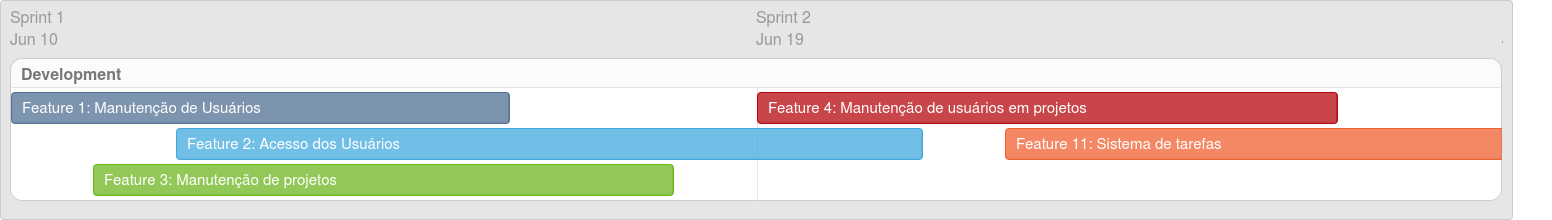
\includegraphics[scale=0.3]{figuras/roadmapPRI}
		\label{img:roadmapPRI}
		\caption{Roadmap Priorizado}
\end{figure}
\FloatBarrier

Como descrito acima, a Feature 2 terá uma parcela entregue na Sprint 1 e uma outra parcela entregue na Sprint 2, garantindo a plena usabilidade das duas parcelas.
O Roadmap completo se encontra no apêndice \ref{sec:roadmap}.

\section{Nível de Time}

O nível de time compreende a camada mais baixa de todo o processo ágil, esta camada é responsável pela implementação da solução técnica, e também pelo detalhamento mais estrito dos requisitos levantados nas camadas superiores, gerando assim as histórias de usuário. O nível de time (Figura \ref{img:programa}) são desempenhadas as seguintes atividades:

\begin{itemize}
\item Levantar User Stories
\item Planejar Sprint
\item Priorizar e detalhar User Stories
\item Desenvolver Sprint
\item Retrospectiva da Sprint
\item Gerenciar User Stories
\end{itemize}

\FloatBarrier
\begin{figure}[!htpd]
		\centering
		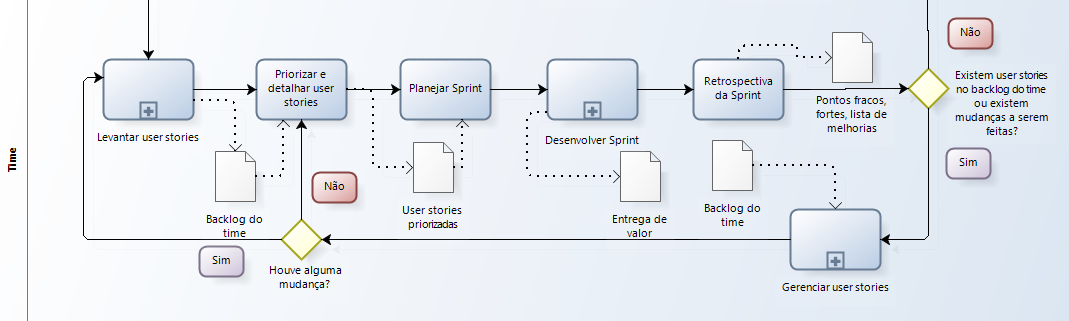
\includegraphics[scale=0.4]{figuras/time}
		\label{img:time}
		\caption{Processo à nível de Time}
\end{figure}

\subsection{Backlog Time}

Logo abaixo é possível verificar as histórias dos usuários, que estão organizadas nos respectivos épicos e features. As histórias seguem o padrão do cartão abaixo.

\FloatBarrier
\begin{table}[!htpd]
\centering
\caption{Modelo do cartão das US}
\label{my-label}
\begin{tabular}{l}
Eu como {[}Ator{]} quero {[}Ação{]} para {[}Funcionalidade{]}
\end{tabular}
\end{table}
\FloatBarrier

Atores identificados:

\begin{itemize}
\item Usuário do sistema
\item Usuário colaborador
\item Gerente de projeto
\item Administrador do Sistema
\end{itemize}

\FloatBarrier
\begin{table}[!htpd]
\centering
\caption{User Story 1}
\label{my-label}
\begin{tabular}{|l|}
\hline
Eu como usuário, quero cadastrar-me no sistema de compartilhamento de projetos. \\ \hline
EP-1 FT-1 US-1                                                                  \\ \hline
Pontos: 3                                                                       \\ \hline
\end{tabular}
\end{table}
\FloatBarrier

\FloatBarrier
\begin{table}[!htpd]
\centering
\caption{User Story 2}
\label{my-label}
\begin{tabular}{|l|}
\hline
\begin{tabular}[c]{@{}l@{}}Eu como usuário, quero alterar meus dados cadastrais para manter \\ meu cadastro atualizado.\end{tabular} \\ \hline
EP-1 FT-1 US-2                                                                                                                       \\ \hline
Pontos: 3                                                                                                                            \\ \hline
\end{tabular}
\end{table}
\FloatBarrier

\FloatBarrier
\begin{table}[!htpd]
\centering
\caption{User Story 3}
\label{my-label}
\begin{tabular}{|l|}
\hline
Eu como usuário, quero excluir minha conta para não ser mais usuário do sistema. \\ \hline
EP-1 FT-1 US-3                                                                   \\ \hline
Pontos: 3                                                                        \\ \hline
\end{tabular}
\end{table}
\FloatBarrier

\FloatBarrier
\begin{table}[!htpd]
\centering
\caption{User Story 4}
\label{my-label}
\begin{tabular}{|l|}
\hline
\begin{tabular}[c]{@{}l@{}}Eu como usuário, quero fazer login no sistema de compartilhamento de projetos para\\ acessar o sistema.\end{tabular} \\ \hline
EP-1 FT-2 US-4                                                                                                                                  \\ \hline
Pontos: 3                                                                                                                                       \\ \hline
\end{tabular}
\end{table}
\FloatBarrier

\FloatBarrier
\begin{table}[!htpd]
\centering
\caption{User Story 5}
\label{my-label}
\begin{tabular}{|l|}
\hline
Eu como usuário, quero fazer logout no sistema para sair do sistema e encerrar a sessão. \\ \hline
EP-1 FT-2 US-5                                                                           \\ \hline
Pontos: 2                                                                                \\ \hline
\end{tabular}
\end{table}
\FloatBarrier

\FloatBarrier
\begin{table}[!htpd]
\centering
\caption{User Story 6}
\label{my-label}
\begin{tabular}{|l|}
\hline
Eu como usuário, quero fazer login pelo Facebook para ter acesso ao sistema. \\ \hline
EP-1 FT-2 US-6                                                               \\ \hline
Pontos: 8                                                                    \\ \hline
\end{tabular}
\end{table}
\FloatBarrier

\FloatBarrier
\begin{table}[!htpd]
\centering
\caption{User Story 7}
\label{my-label}
\begin{tabular}{|l|}
\hline
Eu como usuário, quero fazer login,pelo Google + para ter acesso ao sistema. \\ \hline
EP-1 FT-2 US-7                                                               \\ \hline
Pontos: 8                                                                    \\ \hline
\end{tabular}
\end{table}
\FloatBarrier

\FloatBarrier
\begin{table}[!htpd]
\centering
\caption{User Story 8}
\label{my-label}
\begin{tabular}{|l|}
\hline
\begin{tabular}[c]{@{}l@{}}Eu como criador de projeto, quero criar um projeto para para que ele possa \\ ser desenvolvido no sistema.\end{tabular} \\ \hline
EP-2 FT-3 US-8                                                                                                                                     \\ \hline
Pontos: 3                                                                                                                                          \\ \hline
\end{tabular}
\end{table}
\FloatBarrier

\FloatBarrier
\begin{table}[!htpd]
\centering
\caption{User Story 9}
\label{my-label}
\begin{tabular}{|l|}
\hline
\begin{tabular}[c]{@{}l@{}}Eu como criador do projeto, quero remover um projeto para \\ interromper/impedir o seu desenvolvimento no sistema.\end{tabular} \\ \hline
EP-2 FT-3 US-9                                                                                                                                             \\ \hline
Pontos: 3                                                                                                                                                  \\ \hline
\end{tabular}
\end{table}
\FloatBarrier

\FloatBarrier
\begin{table}[!htpd]
\centering
\caption{User Story 10}
\label{my-label}
\begin{tabular}{|l|}
\hline
\begin{tabular}[c]{@{}l@{}}Eu como criador de projeto, quero editar os dados do projeto \\ para corrigir algum erro de digitação, ou refinar os dados \\ cadastrais do projeto.\end{tabular} \\ \hline
EP-2 FT-3 US-10                                                                                                                                                                              \\ \hline
Pontos: 3                                                                                                                                                                                    \\ \hline
\end{tabular}
\end{table}
\FloatBarrier

\FloatBarrier
\begin{table}[!htpd]
\centering
\caption{User Story 11}
\label{my-label}
\begin{tabular}{|l|}
\hline
\begin{tabular}[c]{@{}l@{}}Eu como criador do projeto, quero aceitar a entrada de \\ contribuidores no projeto para que outras pessoas possam contribuir.\end{tabular} \\ \hline
EP-2 FT-4 US-11                                                                                                                                                        \\ \hline
Pontos: 6                                                                                                                                                              \\ \hline
\end{tabular}
\end{table}
\FloatBarrier

\FloatBarrier
\begin{table}[!htpd]
\centering
\caption{User Story 12}
\label{my-label}
\begin{tabular}{|l|}
\hline
\begin{tabular}[c]{@{}l@{}}Eu como criador do projeto, quero remover contribuidores \\ do projeto para interromper seu acesso ao projeto.\end{tabular} \\ \hline
EP-2 FT-4 US-12                                                                                                                                        \\ \hline
Pontos: 3                                                                                                                                              \\ \hline
\end{tabular}
\end{table}
\FloatBarrier

\FloatBarrier
\begin{table}[!htpd]
\centering
\caption{User Story 13}
\label{my-label}
\begin{tabular}{|l|}
\hline
\begin{tabular}[c]{@{}l@{}}Eu como usuário, quero evoluir de nível no sistema e receber\\ moedas pelas minhas contribuições para que eu permaneça \\ motivado a participar.\end{tabular} \\ \hline
EP-4 FT-5 US-13                                                                                                                                                                          \\ \hline
Pontos: 4                                                                                                                                                                                \\ \hline
\end{tabular}
\end{table}
\FloatBarrier

\FloatBarrier
\begin{table}[!htpd]
\centering
\caption{User Story 14}
\label{my-label}
\begin{tabular}{|l|}
\hline
\begin{tabular}[c]{@{}l@{}}Eu como usuário, quero dar like em um comentário ou tarefa pertinente \\ ao projeto para que quem contribuiu seja motivado pela sua participação, e ganhe moedas.\end{tabular} \\ \hline
EP-4 FT-5 US-14                                                                                                                                                                                           \\ \hline
Pontos: 5                                                                                                                                                                                                 \\ \hline
\end{tabular}
\end{table}
\FloatBarrier

\FloatBarrier
\begin{table}[!htpd]
\centering
\caption{User Story 15}
\label{my-label}
\begin{tabular}{|l|}
\hline
\begin{tabular}[c]{@{}l@{}}Eu como contribuidor, quero dar like em um comentário ou tarefa pertinente \\ ao projeto para que quem contribuiu seja motivado pela sua participação, \\ e ganhe moedas.\end{tabular} \\ \hline
EP-4 FT-5 US-15                                                                                                                                                                                                   \\ \hline
Pontos: 5                                                                                                                                                                                                         \\ \hline
\end{tabular}
\end{table}
\FloatBarrier

\FloatBarrier
\begin{table}[!htpd]
\centering
\caption{User Story 16}
\label{my-label}
\begin{tabular}{|l|}
\hline
\begin{tabular}[c]{@{}l@{}}Eu como criador do projeto, quero dar like em um comentário ou tarefa \\ pertinente ao projeto para que quem contribuiu seja motivado pela sua \\ participação, e ganhe moedas.\end{tabular} \\ \hline
EP-4 FT-5 US-16                                                                                                                                                                                                         \\ \hline
Pontos: 5                                                                                                                                                                                                               \\ \hline
\end{tabular}
\end{table}
\FloatBarrier

\FloatBarrier
\begin{table}[!htpd]
\centering
\caption{User Story 17}
\label{my-label}
\begin{tabular}{|l|}
\hline
\begin{tabular}[c]{@{}l@{}}Eu como usuário, quero visualizar um ranking de projetos para \\ obter um panorama geral dos projetos.\end{tabular} \\ \hline
EP-2 FT-6 US-17                                                                                                                                \\ \hline
Pontos: 6                                                                                                                                      \\ \hline
\end{tabular}
\end{table}
\FloatBarrier

\FloatBarrier
\begin{table}[!htpd]
\centering
\caption{User Story 18}
\label{my-label}
\begin{tabular}{|l|}
\hline
\begin{tabular}[c]{@{}l@{}}Eu como usuário, quero dar like em projetos que acho pertinentes \\ para que o projeto tenha uma visibilidade maior no ranking.\end{tabular} \\ \hline
EP-2 FT-6 US-18                                                                                                                                                         \\ \hline
Pontos: 5                                                                                                                                                               \\ \hline
\end{tabular}
\end{table}
\FloatBarrier

\FloatBarrier
\begin{table}[!htpd]
\centering
\caption{User Story 19}
\label{my-label}
\begin{tabular}{|l|}
\hline
\begin{tabular}[c]{@{}l@{}}Eu como usuário, quero visualizar projetos para obter informações\\ e detalhes do mesmo.\end{tabular} \\ \hline
EP-2 FT-6 US-19                                                                                                                  \\ \hline
Pontos: 2                                                                                                                        \\ \hline
\end{tabular}
\end{table}
\FloatBarrier

\FloatBarrier
\begin{table}[!htpd]
\centering
\caption{User Story 20}
\label{my-label}
\begin{tabular}{|l|}
\hline
\begin{tabular}[c]{@{}l@{}}Eu como criador do projeto, quero solicitar ajuda de outros \\ usuários para esclarecer minhas dúvidas.\end{tabular} \\ \hline
EP-2 FT-6 US-20                                                                                                                                 \\ \hline
Pontos: 6                                                                                                                                       \\ \hline
\end{tabular}
\end{table}
\FloatBarrier

\FloatBarrier
\begin{table}[!htpd]
\centering
\caption{User Story 21}
\label{my-label}
\begin{tabular}{|l|}
\hline
\begin{tabular}[c]{@{}l@{}}Eu como usuário, quero oferecer ajuda para esclarecer dúvidas \\ e contribuir com dúvidas pontuais\end{tabular} \\ \hline
EP-3 FT-7 US-21                                                                                                                            \\ \hline
Pontos: 6                                                                                                                                  \\ \hline
\end{tabular}
\end{table}
\FloatBarrier

\FloatBarrier
\begin{table}[!htpd]
\centering
\caption{User Story 22}
\label{my-label}
\begin{tabular}{|l|}
\hline
\begin{tabular}[c]{@{}l@{}}Eu como criador do projeto, quero vender o projeto para lucrar \\ com as ideias e o valor comercial do projeto.\end{tabular} \\ \hline
EP-3 FT-8 US-22                                                                                                                                         \\ \hline
Pontos: 6                                                                                                                                               \\ \hline
\end{tabular}
\end{table}
\FloatBarrier

\FloatBarrier
\begin{table}[!htpd]
\centering
\caption{User Story 23}
\label{my-label}
\begin{tabular}{|l|}
\hline
\begin{tabular}[c]{@{}l@{}}Eu como criador do projeto, quero transformar o projeto desenvolvido \\ em um produto consolidado para comercializar a ideia desenvolvida.\end{tabular} \\ \hline
EP-3 FT-8 US-23                                                                                                                                                                    \\ \hline
Pontos: 4                                                                                                                                                                          \\ \hline
\end{tabular}
\end{table}
\FloatBarrier

\FloatBarrier
\begin{table}[!htpd]
\centering
\caption{User Story 24}
\label{my-label}
\begin{tabular}{|l|}
\hline                                                                                                                      \begin{tabular}[c]{@{}l@{}}Eu como criador do projeto, quero especificar preço, tipo, descrição, \\ tempo de entrega e forma de pagamento para facilitar a troca a comercialização \\ do produto.\end{tabular} \\ \hline
EP-3 FT-8 US-24                                                                                                                                                                                                \\ \hline
Pontos: 3                                                                                                                                                                                                      \\ \hline
\end{tabular}
\end{table}
\FloatBarrier

\FloatBarrier
\begin{table}[!htpd]
\centering
\caption{User Story 25}
\label{my-label}
\begin{tabular}{|l|}
\hline
Eu como usuário, quero adicionar usuários como amigos para aumentar minha rede de contatos. \\ \hline
EP-1 FT-9 US-25                                                                             \\ \hline
Pontos: 5                                                                                   \\ \hline
\end{tabular}
\end{table}
\FloatBarrier

\FloatBarrier
\begin{table}[!htpd]
\centering
\caption{User Story 26}
\label{my-label}
\begin{tabular}{|l|}
\hline
Eu como usuário, quero excluir amigos para eliminá-los da minha lista de amigos \\ \hline
EP-1 FT-9 US-26                                                                 \\ \hline
Pontos: 5                                                                       \\ \hline
\end{tabular}
\end{table}
\FloatBarrier

\FloatBarrier
\begin{table}[!htpd]
\centering
\caption{User Story 27}
\label{my-label}
\begin{tabular}{|l|}
\hline
\begin{tabular}[c]{@{}l@{}}Eu como usuário, quero seguir outros usuários para receber notificações sobre \\ seus atos, projetos em que participa e suas contribuições.\end{tabular} \\ \hline
EP-1 FT-9 US-27                                                                                                                                                                     \\ \hline
Pontos: 5                                                                                                                                                                           \\ \hline
\end{tabular}
\end{table}
\FloatBarrier

\FloatBarrier
\begin{table}[!htpd]
\centering
\caption{User Story 28}
\label{my-label}
\begin{tabular}{|l|}
\hline
\begin{tabular}[c]{@{}l@{}}Eu como usuário, quero deixar de seguir outros usuários para \\ parar de receber notificações sobre seus atos, projetos em que \\ participa e suas contribuições.\end{tabular} \\ \hline
EP-1 FT-9 US-28                                                                                                                                                                                           \\ \hline
Pontos: 3                                                                                                                                                                                                 \\ \hline
\end{tabular}
\end{table}
\FloatBarrier

\FloatBarrier
\begin{table}[!htpd]
\centering
\caption{User Story 29}
\label{my-label}
\begin{tabular}{|l|}
\hline
\begin{tabular}[c]{@{}l@{}}Eu como usuário, quero pesquisar projetos por nome para\\ encontrar um projeto.\end{tabular} \\ \hline
EP-3 FT-10 US-29                                                                                                         \\ \hline
Pontos: 3                                                                                                               \\ \hline
\end{tabular}
\end{table}
\FloatBarrier

\FloatBarrier
\begin{table}[!htpd]
\centering
\caption{User Story 30}
\label{my-label}
\begin{tabular}{|l|}
\hline
\begin{tabular}[c]{@{}l@{}}Eu como usuário, quero pesquisar projetos por palavras chave \\ para encontrar projetos que estejam em áreas que interessam ao usuário.\end{tabular} \\ \hline
EP-3 FT-10 US-30                                                                                                                                                                \\ \hline
Pontos: 3                                                                                                                                                                       \\ \hline
\end{tabular}
\end{table}
\FloatBarrier

\FloatBarrier
\begin{table}[!htpd]
\centering
\caption{User Story 31}
\label{my-label}
\begin{tabular}{|l|}
\hline
\begin{tabular}[c]{@{}l@{}}Eu como usuário, quero pesquisar projetos por tipo para encontrar \\ projetos pela sua categoria.\end{tabular} \\ \hline
EP-3 FT-10 US-31                                                                                                                          \\ \hline
Pontos: 3                                                                                                                                 \\ \hline
\end{tabular}
\end{table}
\FloatBarrier

\FloatBarrier
\begin{table}[!htpd]
\centering
\caption{User Story 32}
\label{my-label}
\begin{tabular}{|l|}
\hline
\begin{tabular}[c]{@{}l@{}}Eu como usuário, quero acompanhar o desenvolvimento das \\ tarefas do projeto para receber notificações acerca das tarefas.\end{tabular} \\ \hline
EP-2 FT-11 US-32                                                                                                                                                     \\ \hline
Pontos: 6                                                                                                                                                           \\ \hline
\end{tabular}
\end{table}
\FloatBarrier

\FloatBarrier
\begin{table}[!htpd]
\centering
\caption{User Story 33}
\label{my-label}
\begin{tabular}{|l|}
\hline
\begin{tabular}[c]{@{}l@{}}Eu como criador do projeto, quero manter tarefas para que os \\ contribuidores possam contribuir com elas.\end{tabular} \\ \hline
EP-1 FT-9 US-33                                                                                                                                    \\ \hline
Pontos: 4                                                                                                                                          \\ \hline
\end{tabular}
\end{table}
\FloatBarrier

\FloatBarrier
\begin{table}[!htpd]
\centering
\caption{User Story 34}
\label{my-label}
\begin{tabular}{|l|}
\hline
\begin{tabular}[c]{@{}l@{}}Eu como criador do projeto, quero designar tarefas aos colaboradores \\ para que os colaboradores possam cumprir as tarefas designadas.\end{tabular} \\ \hline
EP-2 FT-11 US-34                                                                                                                                                                \\ \hline
Pontos: 7                                                                                                                                                                       \\ \hline
\end{tabular}
\end{table}
\FloatBarrier

\FloatBarrier
\begin{table}[!htpd]
\centering
\caption{User Story 35}
\label{my-label}
\begin{tabular}{|l|}
\hline
\begin{tabular}[c]{@{}l@{}}Eu como usuário, quero desenvolver tarefas do projeto para \\ contribuir com o projeto e receber moedas no sistema.\end{tabular} \\ \hline
EP-2 FT-11 US-35                                                                                                                                            \\ \hline
Pontos: 6                                                                                                                                                   \\ \hline
\end{tabular}
\end{table}
\FloatBarrier

\FloatBarrier
\begin{table}[!htpd]
\centering
\caption{User Story 36}
\label{my-label}
\begin{tabular}{|l|}
\hline
\begin{tabular}[c]{@{}l@{}}Eu como usuário, quero receber notificações de projetos para que \\ eu possa me manter informado sobre atualizações no projeto.\end{tabular} \\ \hline
EP-3 FT-12 US-36 \\ \hline
Pontos: 5                                                                                                                                                               \\ \hline
\end{tabular}
\end{table}
\FloatBarrier

\FloatBarrier
\begin{table}[!htpd]
\centering
\caption{User Story 37}
\label{my-label}
\begin{tabular}{|l|}
\hline
\begin{tabular}[c]{@{}l@{}}Eu como usuário, quero escolher receber notificações do ranking de \\ projetos para me manter atualizado acerca da posição dos projetos.\end{tabular} \\ \hline
EP-3 FT-12 US-37                                                                                                                                                                  \\ \hline
Pontos: 6                                                                                                                                                                        \\ \hline
\end{tabular}
\end{table}
\FloatBarrier

\FloatBarrier
\begin{table}[!htpd]
\centering
\caption{User Story 38}
\label{my-label}
\begin{tabular}{|l|}
\hline
\begin{tabular}[c]{@{}l@{}}Eu como sistema, quero notificar os usuários que estão muito tempo \\ inativos no projeto para que os usuários voltem a acessar o sistema.\end{tabular} \\ \hline
EP-3 FT-12 US-38                                                                                                                                                                    \\ \hline
Pontos: 4                                                                                                                                                                          \\ \hline
\end{tabular}
\end{table}
\FloatBarrier

\FloatBarrier
\begin{table}[!htpd]
\centering
\caption{User Story 39}
\label{my-label}
\begin{tabular}{|l|}
\hline
\begin{tabular}[c]{@{}l@{}}Eu como criador do projeto, quero receber notificações sobre tarefas \\ e comentários realizados no meu projeto para poder monitorá-lo.\end{tabular} \\ \hline
EP-3 FT-12 US-39                                                                                                                                                                 \\ \hline
Pontos: 6                                                                                                                                                                       \\ \hline
\end{tabular}
\end{table}
\FloatBarrier

\FloatBarrier
\begin{table}[!htpd]
\centering
\caption{User Story 40}
\label{my-label}
\begin{tabular}{|l|}
\hline
\begin{tabular}[c]{@{}l@{}}Eu como usuário, quero receber notificações sobre tarefas e comentários \\ realizados no projeto para monitorar o acompanhamento do projeto que \\ estou colaborando.\end{tabular} \\ \hline
EP-3 FT-12 US-40                                                                                                                                                                                               \\ \hline
Pontos: 6                                                                                                                                                                                                     \\ \hline
\end{tabular}
\end{table}
\FloatBarrier

\FloatBarrier
\begin{table}[!htpd]
\centering
\caption{User Story 41}
\label{my-label}
\begin{tabular}{|l|}
\hline
\begin{tabular}[c]{@{}l@{}}Eu como usuário, quero enviar mensagens em um canal de chat \\ para conversar com os usuários do sistema.\end{tabular} \\ \hline
EP-3 FT-13 US-41                                                                                                                                   \\ \hline
Pontos: 10                                                                                                                                        \\ \hline
\end{tabular}
\end{table}
\FloatBarrier

\FloatBarrier
\begin{table}[!htpd]
\centering
\caption{User Story 42}
\label{my-label}
\begin{tabular}{|l|}
\hline
\begin{tabular}[c]{@{}l@{}}Eu como usuário, quero receber mensagens em um canal de chat \\ para conversar com os usuários do sistema.\end{tabular} \\ \hline
EP-3 FT-13 US-42                                                                                                                                    \\ \hline
Pontos: 10                                                                                                                                         \\ \hline
\end{tabular}
\end{table}
\FloatBarrier

\FloatBarrier
\begin{table}[!htpd]
\centering
\caption{User Story 43}
\label{my-label}
\begin{tabular}{|l|}
\hline
\begin{tabular}[c]{@{}l@{}}Eu como usuário, quero criar grupos de bate-papo com os outros \\ usuários do sistema para facilitar a comunicação com várias pessoas.\end{tabular} \\ \hline
EP-3 FT-13 US-43                                                                                                                                                                \\ \hline
Pontos: 10                                                                                                                                                                     \\ \hline
\end{tabular}
\end{table}
\FloatBarrier

\FloatBarrier
\begin{table}[!htpd]
\centering
\caption{User Story 44}
\label{my-label}
\begin{tabular}{|l|}
\hline
\begin{tabular}[c]{@{}l@{}}Eu como usuário, quero visualizar se o usuário para quem \\ estou mandando mensagem está off-line ou online.\end{tabular} \\ \hline
EP-3 FT-13 US-44                                                                                                                                      \\ \hline
Pontos: 5                                                                                                                                            \\ \hline
\end{tabular}
\end{table}
\FloatBarrier

\FloatBarrier
\begin{table}[!htpd]
\centering
\caption{User Story 45}
\label{my-label}
\begin{tabular}{|l|}
\hline
\begin{tabular}[c]{@{}l@{}}Eu como usuário, quero,visualizar se o usuário que estou mandando \\ mensagem está digitando uma mensagem.\end{tabular} \\ \hline
EP-3 FT-13 US-45                                                                                                                                    \\ \hline
Pontos: 10                                                                                                                                         \\ \hline
\end{tabular}
\end{table}
\FloatBarrier

\FloatBarrier
\begin{table}[!htpd]
\centering
\caption{User Story 46}
\label{my-label}
\begin{tabular}{|l|}
\hline
\begin{tabular}[c]{@{}l@{}}Eu como usuário, quero escolher as configurações/preferências da conta \\ no modo default,para que as configurações e preferências da conta voltem \\ ao modo padrão.\end{tabular} \\ \hline
EP-1 FT-14 US-46                                                                                                                                                                                              \\ \hline
Pontos: 8                                                                                                                                                                                                     \\ \hline
\end{tabular}
\end{table}
\FloatBarrier

\FloatBarrier
\begin{table}[!htpd]
\centering
\caption{User Story 47}
\label{my-label}
\begin{tabular}{|l|}
\hline
\begin{tabular}[c]{@{}l@{}}Eu como usuário, quero silenciar todas as notificações para \\ retirar a exibição do som das notificações.\end{tabular} \\ \hline
EP-1 FT-14 US-47                                                                                                                                    \\ \hline
Pontos: 3                                                                                                                                          \\ \hline
\end{tabular}
\end{table}
\FloatBarrier

\FloatBarrier
\begin{table}[!htpd]
\centering
\caption{User Story 48}
\label{my-label}
\begin{tabular}{|l|}
\hline
\begin{tabular}[c]{@{}l@{}}Eu como usuário, quero silenciar apenas as notificações do sistema \\ para retirar a exibição do som das notificações de sistema.\end{tabular} \\ \hline
EP-1 FT-14 US-48                                                                                                                                                           \\ \hline
Pontos: 3                                                                                                                                                                 \\ \hline
\end{tabular}
\end{table}
\FloatBarrier

\FloatBarrier
\begin{table}[!htpd]
\centering
\caption{User Story 49}
\label{my-label}
\begin{tabular}{|l|}
\hline
\begin{tabular}[c]{@{}l@{}}Eu como usuário, quero silenciar apenas as notificações de algum \\ projeto para retirar a exibição do som das notificações de algum projeto.\end{tabular} \\ \hline
EP-1 FT-14 US-49                                                                                                                                                                       \\ \hline
Pontos: 3                                                                                                                                                                             \\ \hline
\end{tabular}
\end{table}
\FloatBarrier

\FloatBarrier
\begin{table}[!htpd]
\centering
\caption{User Story 50}
\label{my-label}
\begin{tabular}{|l|}
\hline
\begin{tabular}[c]{@{}l@{}}Eu como usuário, quero verificar minhas moedas para verificar \\ se minhas contribuições estão sendo importantes para os projetos que contribuo.\end{tabular} \\ \hline
EP-4 FT-15 US-50                                                                                                                                                                          \\ \hline
Pontos: 3                                                                                                                                                                                \\ \hline
\end{tabular}
\end{table}
\FloatBarrier

\FloatBarrier
\begin{table}[!htpd]
\centering
\caption{User Story 51}
\label{my-label}
\begin{tabular}{|l|}
\hline
\begin{tabular}[c]{@{}l@{}}Eu como usuário, quero receber uma moeda, a cada dez likes de \\ usuários que meu comentário receber para verificar se minhas \\ contribuições estão sendo importantes para os projetos que contribuo.\end{tabular} \\ \hline
EP-4 FT-15 US-51                                                                                                                                                                                                                                \\ \hline
Pontos: 4                                                                                                                                                                                                                                      \\ \hline
\end{tabular}
\end{table}
\FloatBarrier

\FloatBarrier
\begin{table}[!htpd]
\centering
\caption{User Story 52}
\label{my-label}
\begin{tabular}{|l|}
\hline
\begin{tabular}[c]{@{}l@{}}Eu como usuário, quero receber uma moeda, por cada likes de colaboradores\\  que meu comentário receber para verificar se minhas contribuições estão sendo \\ importantes para os projetos que contribuo.\end{tabular} \\ \hline
EP-4 FT-15 US-52                                                                                                                                                                                                                                      \\ \hline
Pontos: 4                                                                                                                                                                                                                                            \\ \hline
\end{tabular}
\end{table}
\FloatBarrier

\FloatBarrier
\begin{table}[!htpd]
\centering
\caption{User Story 53}
\label{my-label}
\begin{tabular}{|l|}
\hline
\begin{tabular}[c]{@{}l@{}}Eu como criador do projeto quero conceder uma moeda por colaboração \\ para motivar usuários a colaborarem com sugestões construtivas.\end{tabular} \\ \hline
EP-4 FT-15 US-53                                                                                                                                                                \\ \hline
Pontos: 4                                                                                                                                                                      \\ \hline
\end{tabular}
\end{table}
\FloatBarrier

\FloatBarrier
\begin{table}[!htpd]
\centering
\caption{User Story 54}
\label{my-label}
\begin{tabular}{|l|}
\hline
\begin{tabular}[c]{@{}l@{}}Eu como administrador, quero cancelar contas de usuários que \\ não estão fazendo uso devido do sistema.\end{tabular} \\ \hline
EP-1 FT-16 US-54                                                                                                                                 \\ \hline
Pontos: 3                                                                                                                                        \\ \hline
\end{tabular}
\end{table}
\FloatBarrier

\FloatBarrier
\begin{table}[!htpd]
\centering
\caption{User Story 55}
\label{my-label}
\begin{tabular}{|l|}
\hline
Eu como administrador, quero receber denúncias de usuários do sistema. \\ \hline
EP-1 FT-16 US-55                                                       \\ \hline
Pontos: 8                                                              \\ \hline
\end{tabular}
\end{table}
\FloatBarrier

\FloatBarrier
\begin{table}[!htpd]
\centering
\caption{User Story 56}
\label{my-label}
\begin{tabular}{|l|}
\hline
Eu como administrador, quero aplicar atualizações no sistema. \\ \hline
EP-1 FT-16 US-56                                               \\ \hline
Pontos: 8                                                     \\ \hline
\end{tabular}
\end{table}
\FloatBarrier

\FloatBarrier
\begin{table}[!htpd]
\centering
\caption{User Story 57}
\label{my-label}
\begin{tabular}{|l|}
\hline
\begin{tabular}[c]{@{}l@{}}Eu como administrador, quero monitorar o sistema recebendo \\ mensagens dos usuários.\end{tabular} \\ \hline
EP-1 FT-16 US-57                                                                                                               \\ \hline
Pontos: 6                                                                                                                     \\ \hline
\end{tabular}
\end{table}
\FloatBarrier

\section{Gerência de Mudança}

\subsection{Atributos de Requisitos}

De forma a contribuir na identificação e na obtenção de informações mais detalhadas dos requisitos dentro do projeto, foi realizada uma identificação por atributos nestes, dentro da plataforma, de forma a identificar rastreabilidade, progresso, prioridade e risco dentro do projeto.

\subsubsection{Origem}

De forma a garantir a rastreabilidade e origem dos requisitos, os atributos foram identificados de acordo com a seguinte tabela:

\FloatBarrier
\begin{table}[\htp]
\centering
\caption{Atributos do requisito}
\label{my-label}
\begin{tabular}{|l|l|l}
\cline{1-2}
EP & Épico      &  \\ \cline{1-2}
FT & Feature    &  \\ \cline{1-2}
US & User Story &  \\ \cline{1-2}
\end{tabular}
\end{table}
\FloatBarrier

\FloatBarrier
\begin{figure}[!htpd]
		\centering
		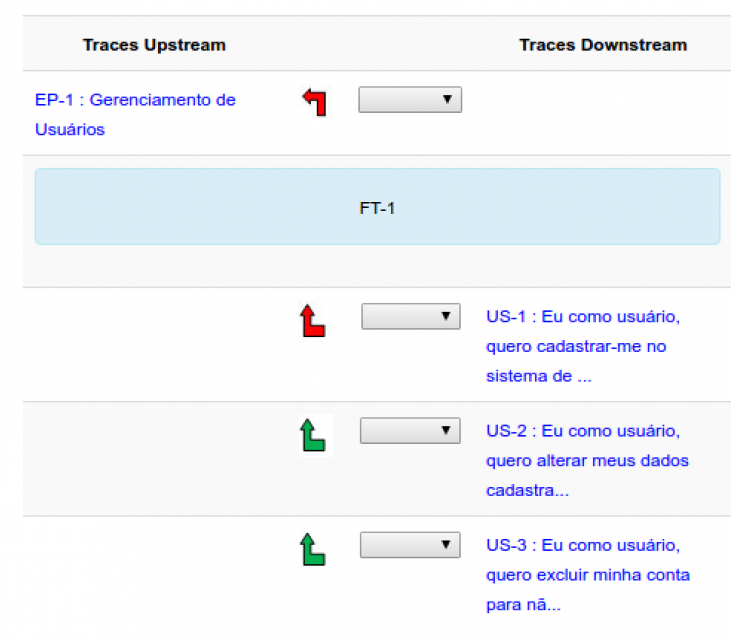
\includegraphics[scale=0.4]{figuras/origem}
		\label{img:origem}
		\caption{Atributo do requisito - Origem}
\end{figure}
\FloatBarrier

\subsubsection{Status}

Visando monitorar o grau de completude do requisito, foi utilizado um atributo de Status do requisito, em forma de porcentagem.

\FloatBarrier
\begin{figure}[!htpd]
		\centering
		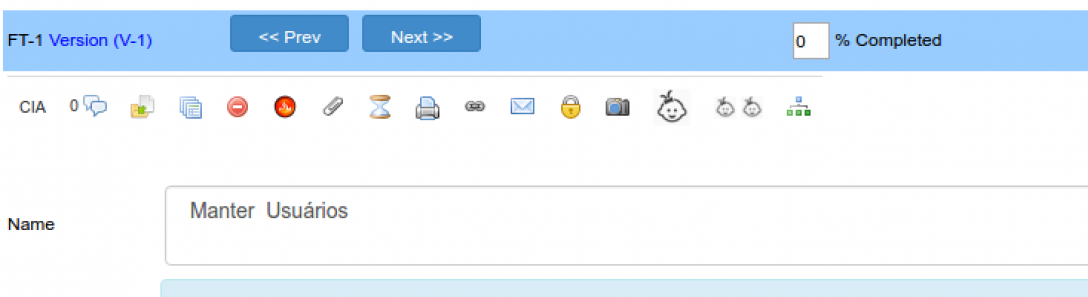
\includegraphics[scale=0.4]{figuras/status}
		\label{img:status}
		\caption{Atributo do requisito - Status}
\end{figure}
\FloatBarrier

\subsubsection{Prioridade}

Para caracterizar a prioridade dos requisitos, eles foram classificado entre prioridade média, alta ou baixa, de forma a evidenciar sua importância no contexto do projeto.

\FloatBarrier
\begin{figure}[!htpd]
		\centering
		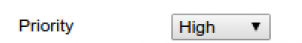
\includegraphics[scale=0.4]{figuras/prioridade}
		\label{img:prioridade}
		\caption{Atributo do requisito - Prioridade}
\end{figure}
\FloatBarrier

\subsubsection{Complexidade}

De forma a ter um controle de tempo de entrega dos requisitos, foi atribuído ainda o nível de complexidade deste, de forma a permitir um maior controle de data de entrega. Tal classificação tem 3 níveis: Baixa, Média e Alta. É feita a atribuição na descrição do requisito.

\subsubsection{Risco}

Caracteriza o risco que a implementação deste requisito traz para a integridade do projeto. Também classificado em 3 níveis: Baixo, Médio e Alto e também atribuído na descrição do requisito.

\FloatBarrier
\begin{figure}[!htpd]
		\centering
		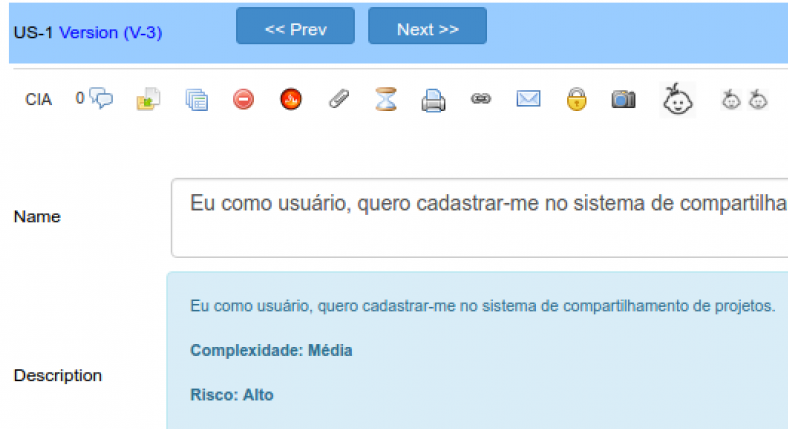
\includegraphics[scale=0.4]{figuras/risco}
		\label{img:risco}
		\caption{Atributo do requisito - Risco}
\end{figure}
\FloatBarrier

\section{Rastreabilidade}

Rastreabilidade define-se, segundo Edwards, como sendo a técnica usada para prover relacionamento entre requisitos, arquitetura e implementação final do sistema \cite{ed}. Ela auxilia ainda na compreensão dos relacionamentos existentes entre requisitos do software ou entre artefatos de requisitos, arquitetura e implementação. Esses relacionamentos permitem aos projetistas mostrar que o projeto atende aos requisitos. A rastreabilidade também apóia a detecção precoce daqueles requisitos não atendidos pelo software \cite{palmer}.

\FloatBarrier
\begin{figure}[!htpd]
		\centering
		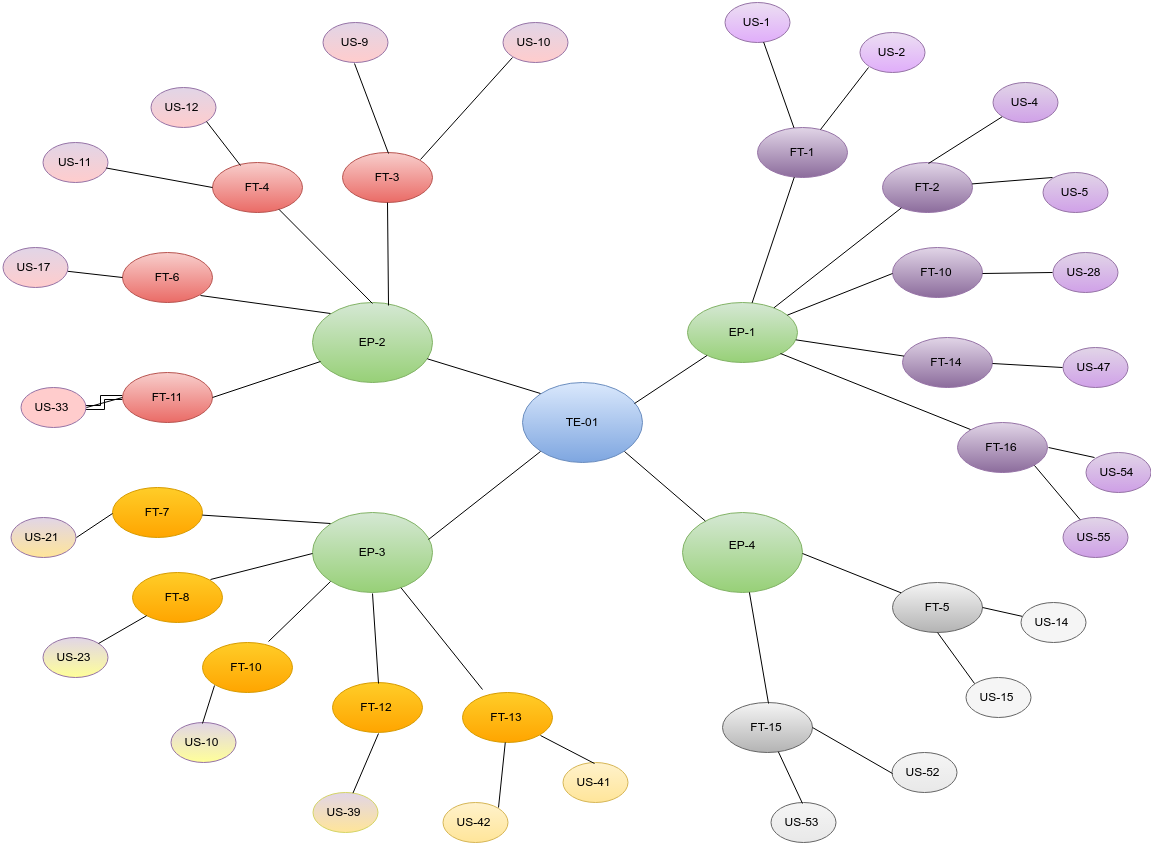
\includegraphics[scale=0.4]{figuras/Rastreabilidade}
		\label{img:rastreabilidade}
		\caption{Rastreabilidade}
\end{figure}
\FloatBarrier

A rastreabilidade foi foi documentada na ferramenta Tracecloud como se segue:

\FloatBarrier
\begin{figure}[!htpd]
		\centering
		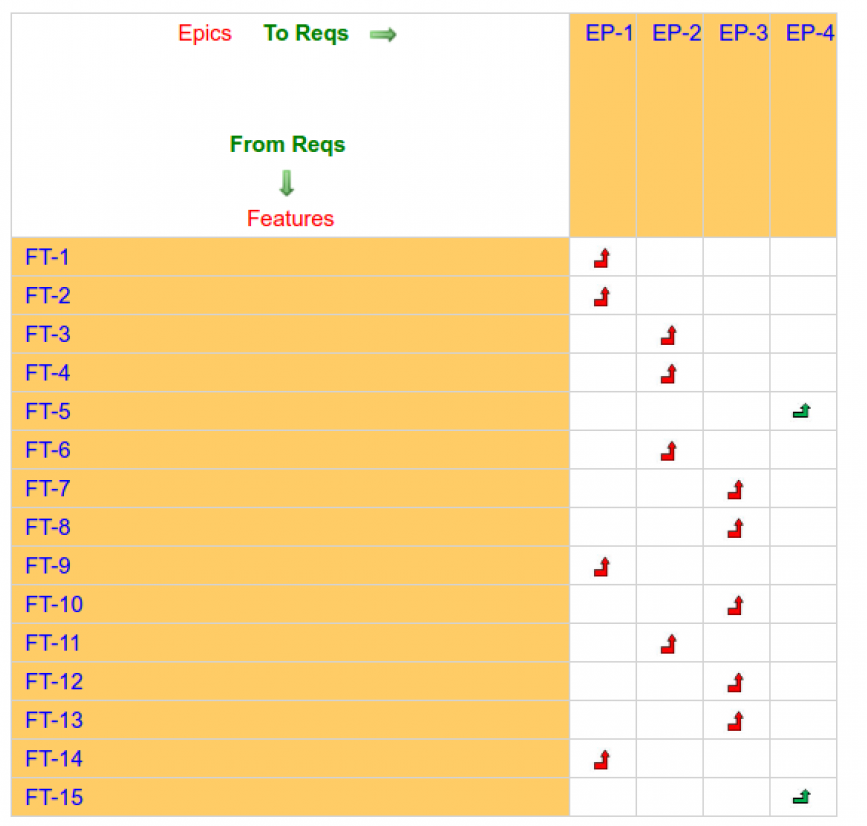
\includegraphics[scale=0.4]{figuras/rast1}
		\label{img:rast1}
		\caption{Rastreabilidade dos Requisitos (Épicos - Features)}
\end{figure}
\FloatBarrier

\FloatBarrier
\begin{figure}[!htpd]
		\centering
		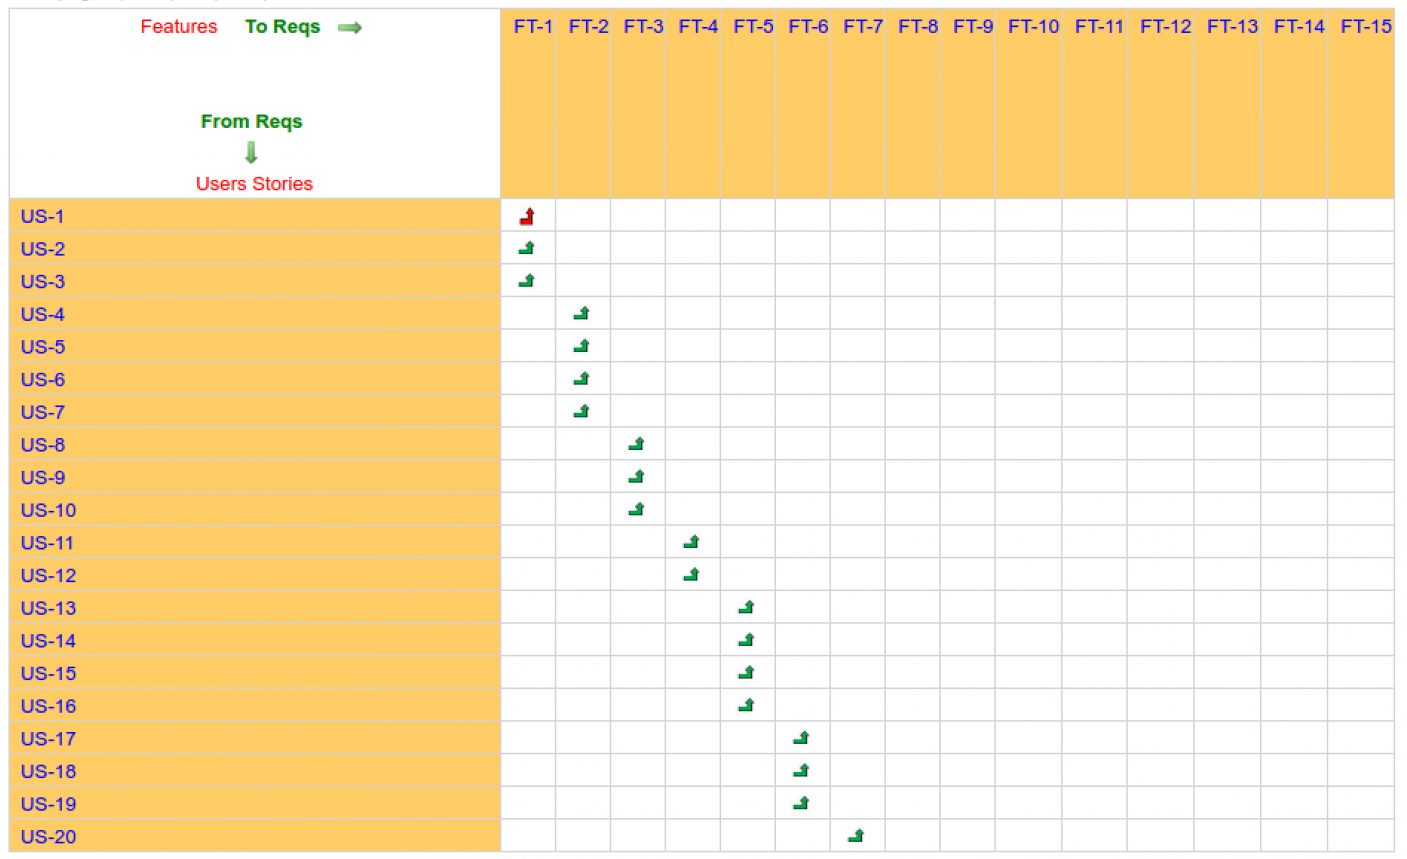
\includegraphics[scale=0.25]{figuras/rast2}
		\label{img:rast2}
		\caption{Rastreabilidade dos Requisitos (Features - User Stories)}
\end{figure}
\FloatBarrier

\FloatBarrier
\begin{figure}[!htpd]
		\centering
		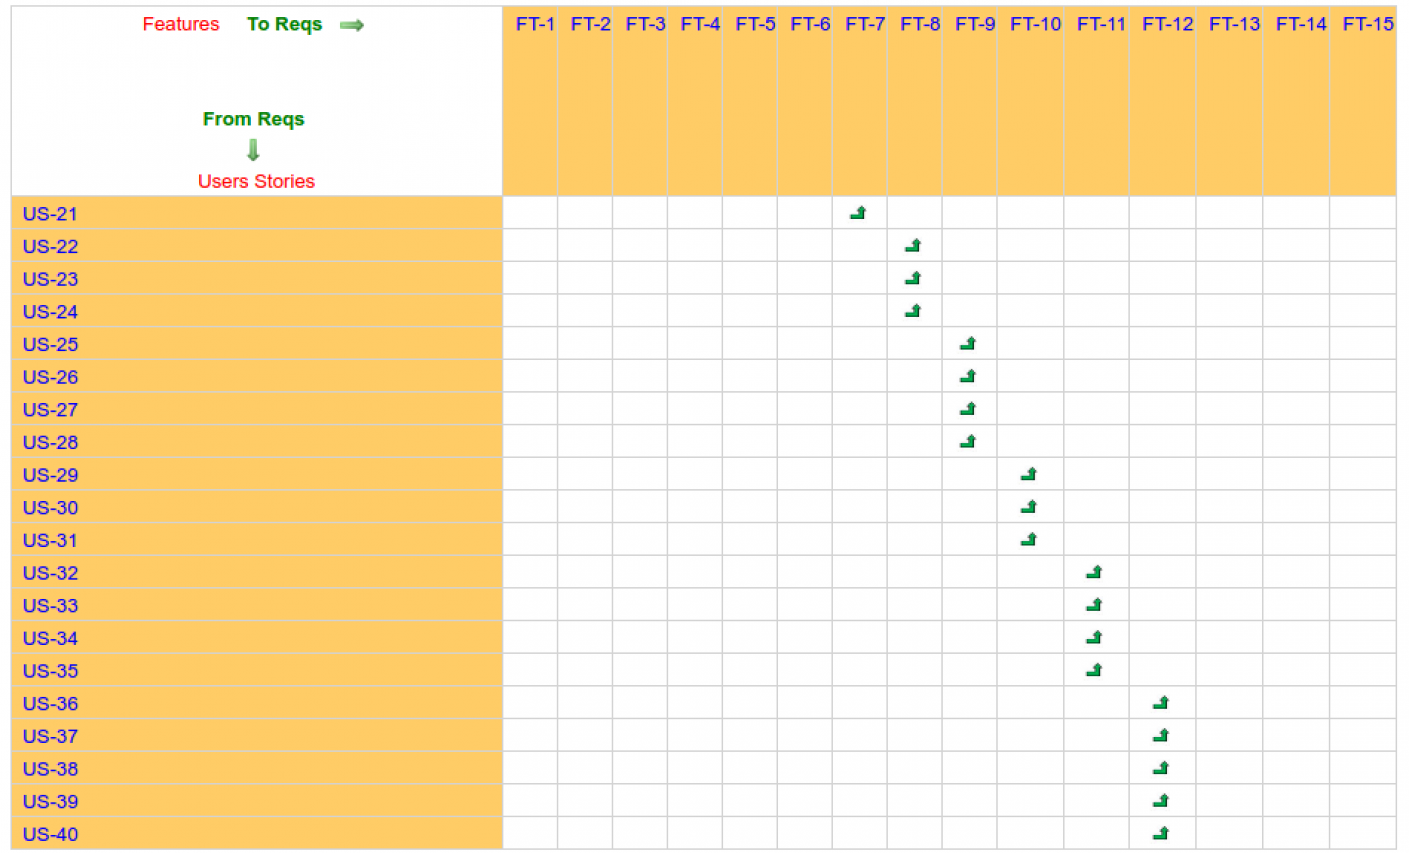
\includegraphics[scale=0.25]{figuras/rast3}
		\label{img:rast3}
		\caption{Rastreabilidade dos Requisitos completa (Features - User Stories)}
\end{figure}
\FloatBarrier
